\documentclass[10pt]{article}
\usepackage[utf8]{inputenc}
\usepackage{graphicx}

\title{CC0504 - Sistemas Operacionais}
\author{Guilherme Vasconcelos}
\date{Abril 2019}
\begin{document}
\maketitle

\section{Introdução}
\ A Disciplina de Sistemas Operacionais tem como principal objetivo capacitar o aluno a entender a arquitetura conceitual e o funcionamento geral dos principais componentes dos sistemas operacionais modernos. Primeiramente aprende-se os conceitos basicos de SO(Sistema Operacional) que seria: Abstração e gerência de recursos, funcionalidades, estrurura e arquitetura de SOs entre outros topicos. Essa disciplina é inserida em tecinicas basicas de computação e em Matérias essenciais para formação especifica em computação.~\cite{einstein}

\begin{figure}[!htb]
    \centering
    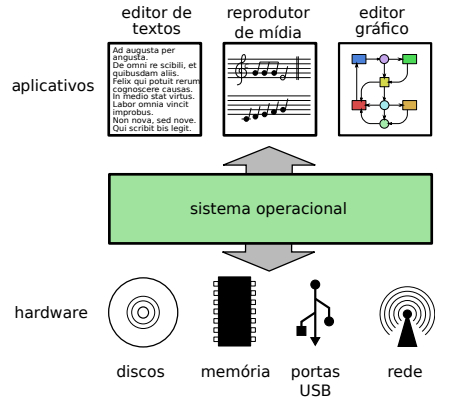
\includegraphics[scale=0.7]{visao2.png}
    \caption{Visão geral de um Sistema Operacional}
    \end{figure}
    
\section{Relevância}
\ Os sistemas operacionais são elementos fundamentais para o funcionamento de praticamente qualquer sistema de computação, dos minúsculos sistemas embarcados e telefones celulares aos gigantescos centros de processamento de dados das grandes empresas. Apesar da imensa diversidade de sistemas operacionais existentes, eles tentam resolvem problemas de mesma natureza e seguem basicamente os mesmos princípios.

Conhecer Sistemas Operacionais a fundo não é algo reservado a hackers, mas importante para todo profissional de computação, pois os mecanismos implementados pelo sistema operacional afetam diretamente o comportamento e o desempenho das aplicações. Além disso, o sistema operacional é uma peça chave na configuração de serviços de rede e na segurança do sistema.~\cite{lisa}

\textbf{Pontos positivos:} Entender a estrutura, funcionalidade, arquitetura entre outros temas sobre Sistemas Operacionais

\textbf{Pontos negativos:} Muitas informações especificas e a dificuldade de acompanhar novas informações.

\section{Relação com outras disciplinas}

A tabela \ref{tab1}

\begin{table}[!htb]
\label{tab1}
\begin{tabular}{ll}
CC0851 - Segurança de Dados    & \begin{tabular}[c]{@{}l@{}}Disciplina Optativa inclusa em Ciência de Dados que tem como \\ pre-requisito Sistemas Operacionais, já que para proteger informações \\ Eletrônicas é necessário compreender o sistema operacional e \\ suas funções e assim usar dele para melhor segurança das informações \\ do usuário.\end{tabular} \\  
\\

CC0852 - Sistemas Distribuidos & \begin{tabular}[c]{@{}l@{}}Disciplina Optativa inclusa em redes e comunicações que tem como \\ pre-requisito Sistemas Operacionais, já que basicamente o aluno irá \\ aprender a desenvolver uma aplicação\\ simples, de forma distribuída, utilizando os conceitos e ferramentas \\ usadas também  por um sistema operacional.\end{tabular} ~\cite{albert}
\end{tabular}
\end{table}

\bibliographystyle{ieeetr}
\bibliography{referencias.bib}


\end{document}


